\section{Filtrado de señales}
	\subsection{}
		Acerca del filtro se tiene la siguiente información:
		\begin{enumerate}
			\item Es un filtro pasa-alto y tiene un polo en cero
			\item El polo está ubicado a una distancia $r = 0.9$ del origen en el plano-z
			\item Las señales constantes no pasan por el sistema
		\end{enumerate}
		
		A partir de los datos, se puede deducir que se tiene un rechazo para DC, por lo que la ubicación del cero en el plano complejo debe cumplir:
		\begin{equation*}
			z - 1 = 0 \Longleftrightarrow z = 1
		\end{equation*}
		
		Sabiendo que $z = e^{j\omega}$, al evaluar en $\omega = 0$ se tendrá rechazo de la banda DC. Para la ubicación del polo, se sabe conviene que este esté lo más apegado al cero, de esta forma se tendrá un filtro con mayor selectividad, se comportara como un filtro \textit{notch} 	para DC. Por lo que podemos definir la ubicación del polo en $z_{p} = 0.9$. De esta forma la función de transferencia queda de la siguiente forma:
		\begin{equation}
		H(z) = \frac{z-1}{z-0.9}
		\label{eq:1_filter_transfer_function}
		\end{equation}
		
		Realizando el diagrama de polos y ceros:
		\begin{figure}[H]
			\center
			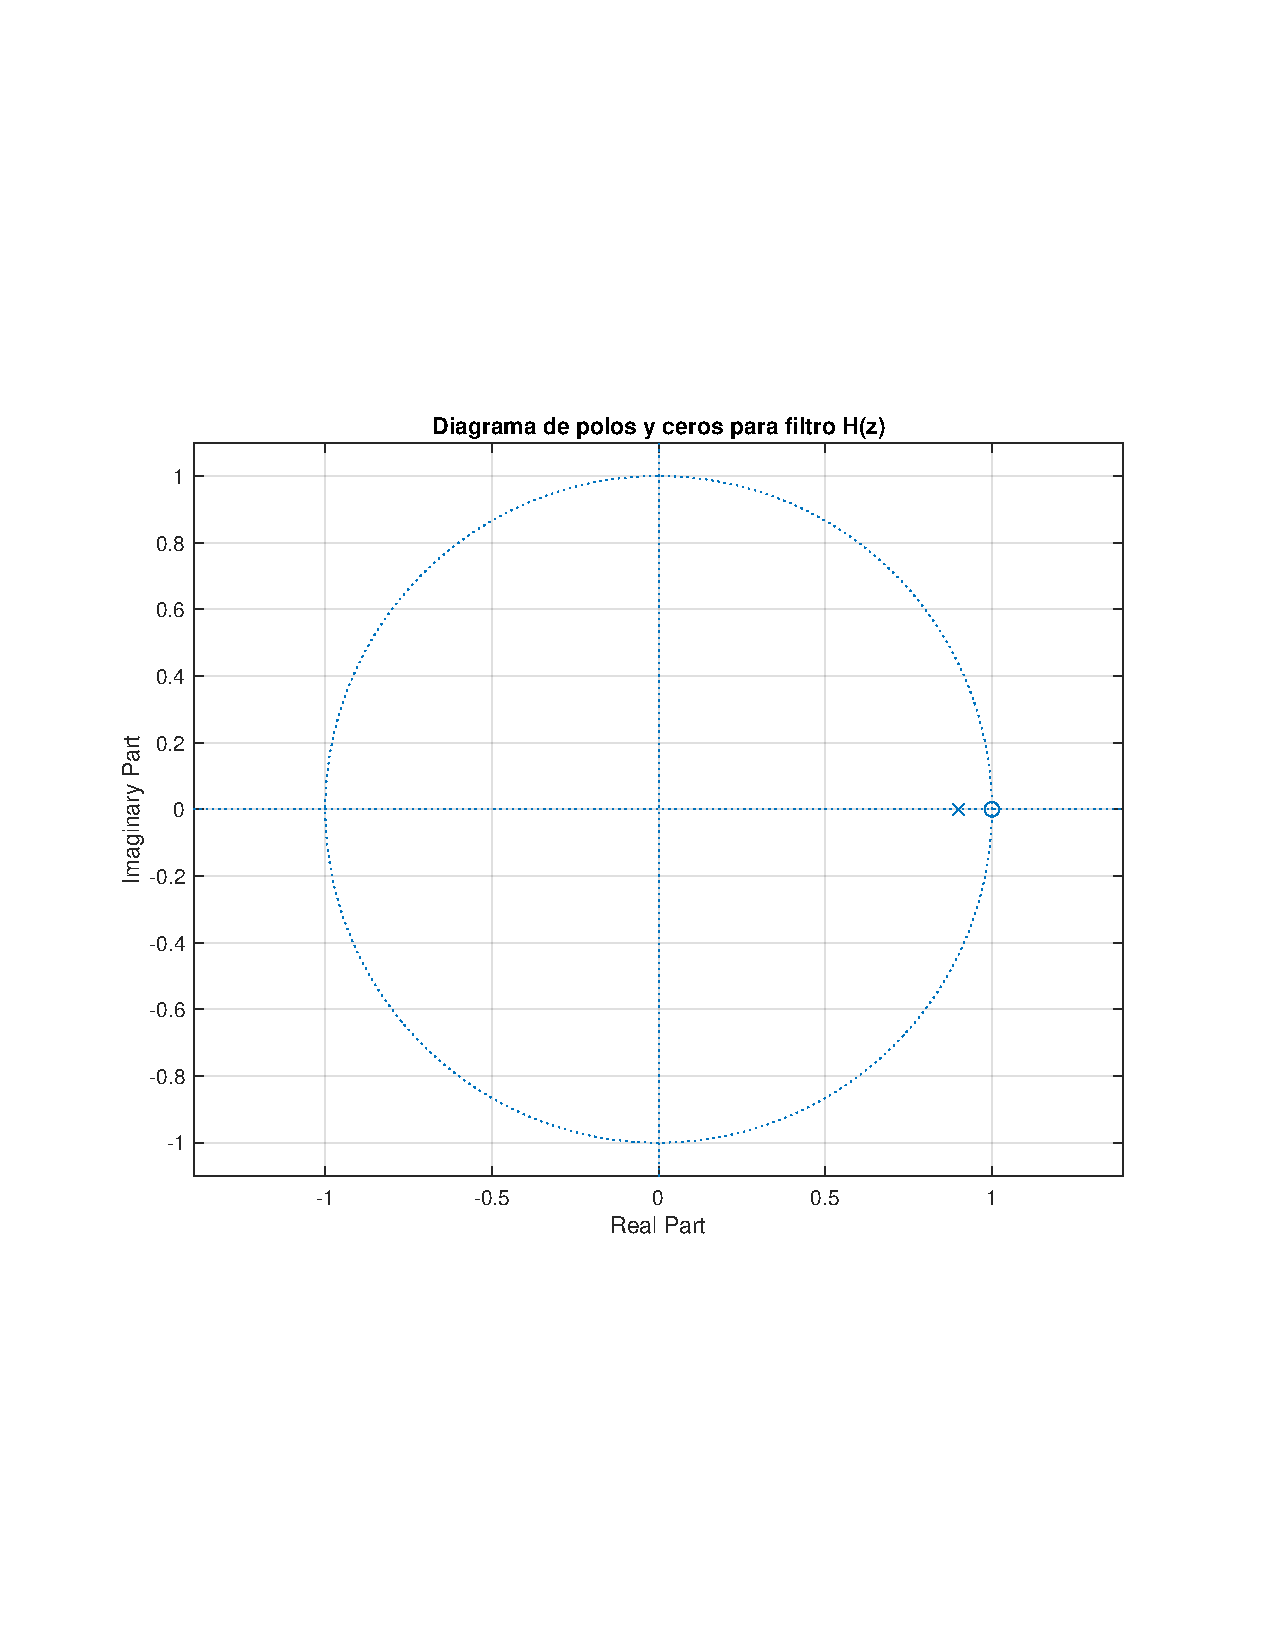
\includegraphics[width=0.6\textwidth,clip, trim = {1.9cm 6.8cm 2.3cm 7cm}]{../plots/1_zp_diag.pdf}
			\caption{Diagrama de polos y ceros para la función de transferencia \ref{eq:1_filter_transfer_function}}
			\label{fig:1_zero_pole_diagram}
		\end{figure}
		
		Analizando la respuesta en magnitud y fase del filtro:
		\begin{figure}[H]
			\center
			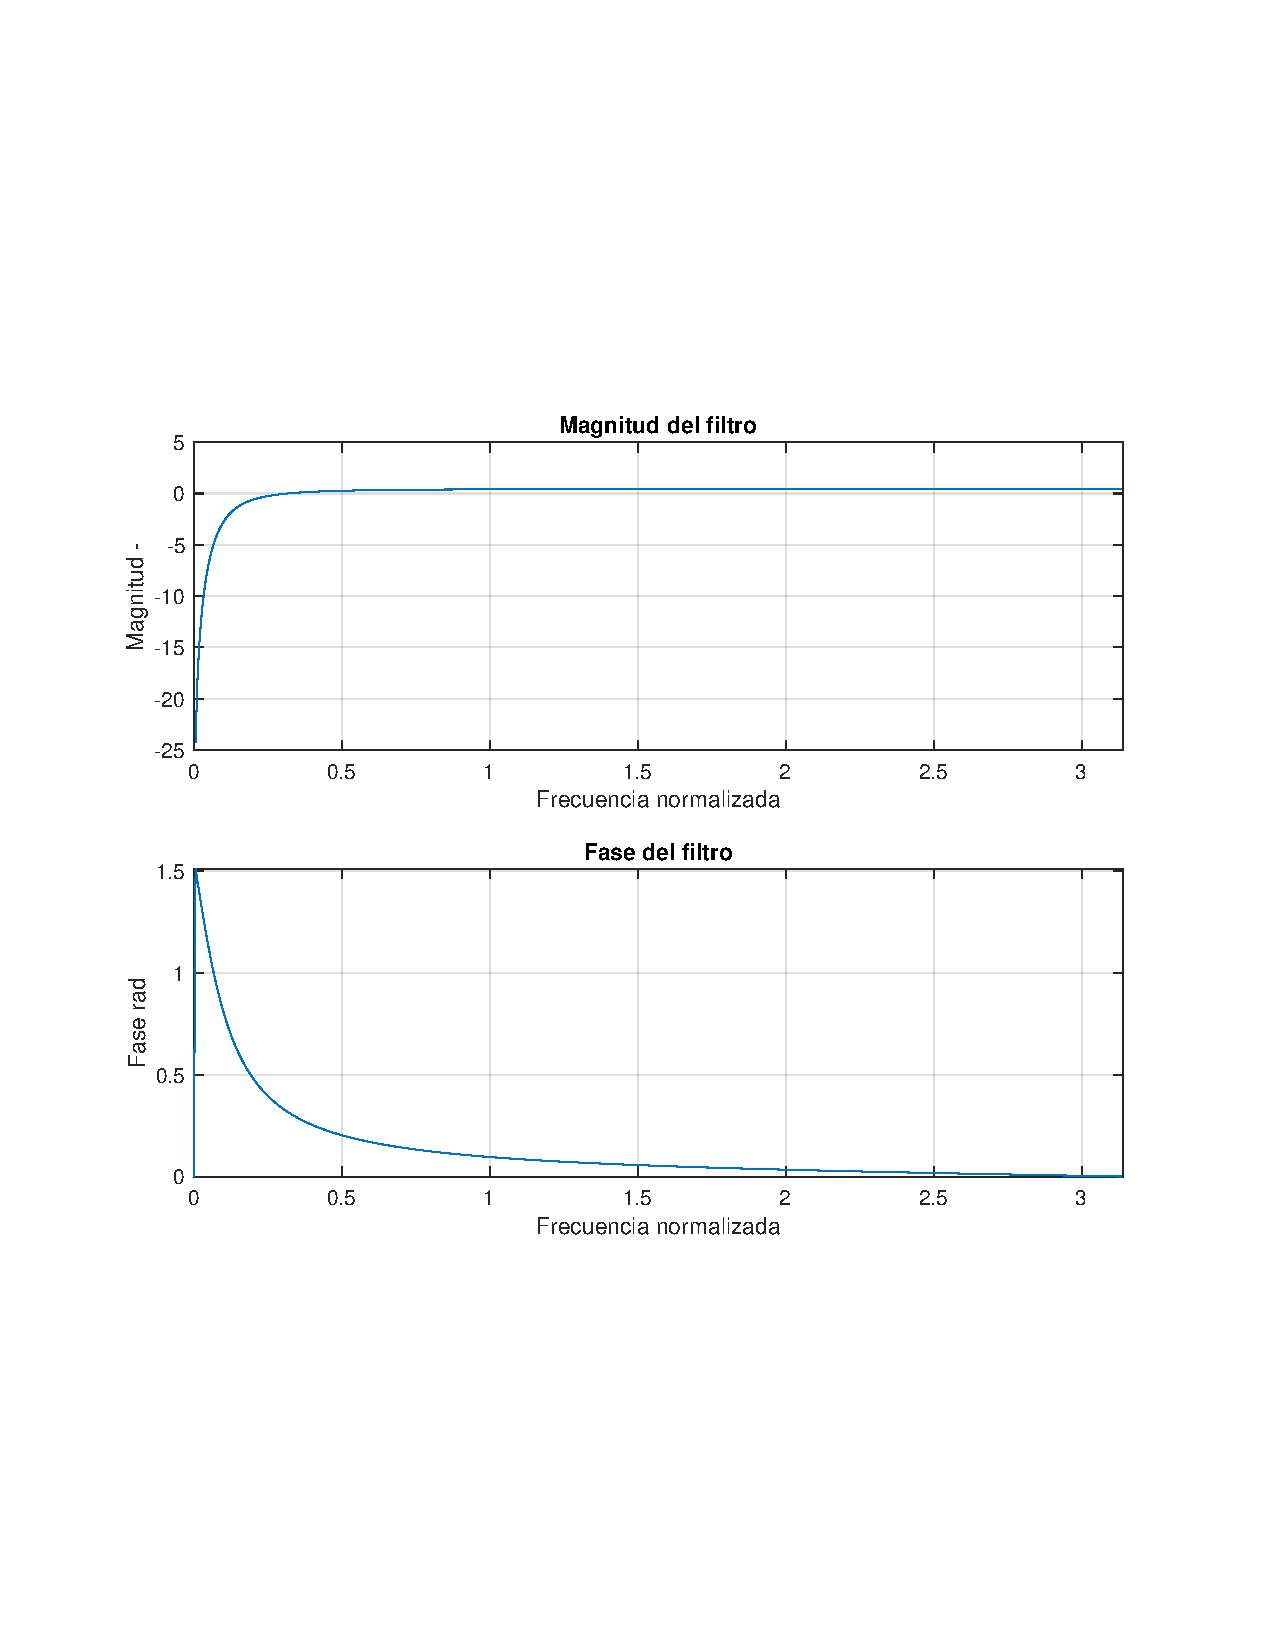
\includegraphics[width=0.6\textwidth,clip, trim = {1.9cm 6.8cm 2.3cm 7cm}]{../plots/1_mag_phase.pdf}
			\caption{Respuesta en magnitud y fase para el filtro}
		\end{figure}
		
		Se procede a evaluar la función \ref{eq:1_filter_transfer_function}, para $\omega = pi$:
		
		\begin{equation}
			H(\pi) = \frac{e^{j\pi} - 1}{e^{j\pi} - 0.9} = \frac{-2}{-1,9} \approx 1.0526
			\label{eq:1_filter_pi}
		\end{equation}
		
		Para normalizar la respuesta del filtro, para $\omega = \pi$, basta con hacer que para esta frecuencia el filtro tenga ganancia unitaria, por lo que se puede definir la ganancia de normalización:
		\begin{equation}
			G_{n} = \frac{1.9}{2} = 0.95
		\end{equation}
		
		Por lo que se puede reescribir la función de transferencia:
		\begin{equation}
			\hat{H}(z) = G_{n} \cdot H(z) = 0.95 \cdot \frac{z - 1}{z -0.9} 
			\label{eq:1_transfer_function_normal}
		\end{equation}
		
		Llevando la expresión a su forma de ecuación de diferencias:
		\begin{align}
			X(z) \cdot 0.95 ( 1 - z^{-1} ) = Y(z) \cdot (1 - 0.9 z^{-1}) \\
			y(z) = 0.9 \cdot y\left[ n - 1 \right] + 0.95 \left( x\left[ n - 1 \right] - x\left[n \right] \right)
		\end{align}
		
		
			